\documentclass[11pt]{article} 

\usepackage{fullpage}
\usepackage{fancybox}
%\usepackage{oz}
\usepackage{multicol}
\usepackage{ifthen}
\usepackage{version}
\usepackage{url}
\usepackage{amsfonts}
\usepackage{amsmath}
\usepackage{graphicx}
\usepackage{enumerate}
\usepackage{booktabs}
\usepackage{hyperref}

\newlength{\tab}
\setlength{\tab}{1em}
\setlength{\parindent}{0pt}
\setlength{\parskip}{6pt}
\setlength{\evensidemargin}{0.0cm}
\setlength{\oddsidemargin}{0.0cm}
\setlength{\textwidth}{16cm}
%  \setlength{\headsep}{0cm}
\setlength{\headheight}{0cm}
\setlength{\topmargin}{0cm}
\setlength{\textheight}{23cm}
\setlength{\itemsep}{0pt}
\setlength{\topsep}{0pt}


\definecolor{javared}{rgb}{0.6,0,0} % for strings
\definecolor{javagreen}{rgb}{0.25,0.5,0.35} % comments
\definecolor{javapurple}{rgb}{0.5,0,0.35} % keywords
\definecolor{javadocblue}{rgb}{0.25,0.35,0.75} % javadoc
\definecolor{javabackground}{rgb}{0.9,0.9,0.9}
\definecolor{javablack}{rgb}{0,0,0}

\lstset{language=Ada,
  backgroundcolor=\color{javabackground},
  basicstyle=\ttfamily\fontsize{10}{12}\selectfont,
  keywordstyle=\color{javablack}\bfseries,
  aboveskip={1.5\baselineskip},
  stringstyle=\color{javared},
  commentstyle=\color{javagreen},
  morecomment=[s][\color{javadocblue}]{/**}{*/},
  numbers=left,
  numberstyle=\tiny\color{black},
  frame=single,
  numbersep=10pt,
  stepnumber=1,
  tabsize=8,
  xleftmargin=0ex,
  xrightmargin=0ex,
  showspaces=false,
  showstringspaces=false,
  aboveskip=0.5ex
}


\usepackage[textsize=scriptsize,textwidth=1cm]{todonotes}
\newcommand{\tm}[1]{\todo[inline,color=yellow]{#1}}
%=======================================================================
%      New Environments
%
\newtheorem{definition}{Definition}
\newtheorem{theorem}[definition]{Theorem}
\newtheorem{proposition}[definition]{Proposition}
\newtheorem{lemma}[definition]{Lemma}
\newtheorem{remark}[definition]{Remark}
\newtheorem{exercise}[definition]{Exercise}
\newtheorem{example}[definition]{Example}

\newenvironment{omitable}[1]{}

%----------------------------------------------------------------------
%    The Document
%

\newcommand{\assignmenttitle}[2]{
\begin{center}
\textbf{\sc The University of Melbourne}\\[0.5ex]
\textbf{\sc SWEN90010: High Integrity Software Engineering}\\[1ex]
\textbf{\large Assignment {#1}}\\[1ex]
%\textbf{\sc Second Semester, 2014}\\[1ex]
\textbf{\sc Due Date: #2}
\end{center}
}


\newcommand{\solutionstitle}[2]{
\mbox{}\\
%\vspace{10ex}
\begin{center}n
\textbf{\sc The University of Melbourne}\\[0.5ex]
\textbf{\sc SWEN90010: High Integrity Software Engineering}\\[1ex]
\textbf{\large Assignment {#1} Solutions}\\[1ex]
%\textbf{\sc Second Semester, 2014}\\[1ex]
\textbf{\sc Due Date: #2}
\end{center}
\vspace{5ex}
}


\begin{document}

\assignmenttitle{1}{11:59pm, Sunday 20 March, 2016}

\section{Introduction}

This assignment is worth 10\% of your total mark.

The aim of this assignment is to provide you with an opportunity to implement a simplified safety- and security-critical system in Ada. Doing so will help to explore the properties of Ada, and how they relate to safe programming.

\textbf{Tip:} Perhaps the most difficult part of this assignment is getting your head around the system itself, and the packages already supplied. Be sure to read this carefully before you start, and to understand the example scenario and how its uses the interfaces of the supplied packages.


\section{System overview}

The system to be produced as part of the assignment is part of a fictional fitness monitoring device called the \emph{FatBat}\footnote{This device is fictitious and any similarity to existing products is entirely coincidental}.

A FatBat looks like a wristwatch and includes functions for monitoring the wearer's health and uploading this information into a cloud-based system.  It monitors heart rate and uses {GPS} locations and  footsteps to measure a person's activity and fitness. Figure~\ref{fig:fatBat}\footnote{Image from flickr, reused under Creative Commons} shows a picture of a FatBat.


\begin{figure}[!h]
 \centering
 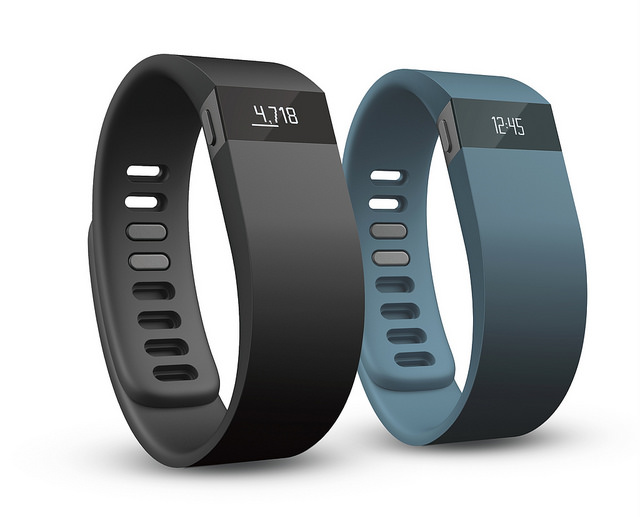
\includegraphics[scale=0.8]{./figs/fatBat}
 \caption{FatBat fitness and health monitor}
 \label{fig:fatBat}
\end{figure}

The FatBat has four intended features:
\begin{enumerate}
        \item to record a person's vital signs
	\item to phone 000 when a person suffers from a cardiac arrest (as judged by irregularities in heart beat),
	\item to share some limited information with an insurance company, in order to reduce premiums, and
	\item to share information with friends for social reasons; {\it e.g. } competitions to see who can take the most steps.
\end{enumerate}

Each FatBat's data is stored in the cloud.  Each user can set access permissions to their own data, described below.

Your aim is to design a sub-system of the FatBat and its cloud storage that communicates just the right amount of information to just the right places at the right times.

\section{Requirements}
\label{sec:requirements}

\subsection{Roles}

There are four roles that take part in this system:

\begin{enumerate}

 \item \emph{Wearer}: The user identity (\texttt{UID}) of the person wearing the FatBat.

 \item \emph{Emergency}: The Emergency services, contacted by calling 000.

 \item \emph{Insurance}: The user's insurance company.
 
 \item \emph{Social}: The user's friends.
 
\end{enumerate}



\subsection{Data}
Each FatBat has a user id \texttt{UID} and three types of personal data:
\begin{enumerate}
	\item an internal \texttt{GPS} locator,
	\item a daily \texttt{footsteps} count, and
%	\item \emph{GPS} It also records {GPS} location every ten minutes, and stores 7 days' data.   
	\item \texttt{heart monitor}, a bit indicating whether the person is having a heart attack.
\end{enumerate}

It also has two user-set bits, each with some attached information.
\begin{enumerate}
	\item {\bf Insurance:} \texttt{(insured, InsuranceCo)}.    
	\item {\bf Social:} A list of  \texttt{(UID, footsteps, {GPS}, heartmonitor)} tuples.  The UID indicates another FatBat user, with whom this user wants to share data.  Permissions are indicated by setting the bits \texttt{footsteps}, \texttt{GPS} and \texttt{heartmonitor} to indicate that the person with the given UID is allowed to read that data.
\end{enumerate}

\subsection{Intended Communications}

The FatBat is supposed to support three different kinds of communication:

\begin{enumerate}[~~\bf{R1}.1]
	\item At 11:59pm every day, the FatBat uploads the total day's footsteps.  (Keeping a continuing record of the last 30 days.)
	\item At ten-minute intervals, the FatBat updates its {GPS} location.

  \item \texttt{Emergency}: If the wearer experiences a heart attack, the FatBat should call 000 and report the current {GPS} coordinates. 
  
  \item \texttt{Insurance}: If the \texttt{insured} bit is set, the specified insurance company may read that person's footsetps.

  \item \texttt{Social}: Each person in the list of friends may read the data for which the corresponding bit is set.

	\item \texttt{OwnMonitoring}: Each person may read their own data.
 % Precondition for switching.


\end{enumerate}

Extra:  (VT: not quite written out.  I'm not so sure this fits clearly any more - see how you go implementing it.:) You can give permission for 000 calls, which are off by default.  It shares your location with 000 if you've shared your vitals with them and you call.  

\section{Your tasks}

 Implement an Ada package called \texttt{FatBat}, which implements the functionality described in ``Intended Communications,'' using the following functions:
\begin{itemize}
\item \texttt{Adduser(UID)}: 
\item \texttt{AddInsuranceCompany(my-UID, insurance-UID)}:
\item \texttt{Addfriends(my-UID, friend-UID)}:
\item \texttt{AssignInsurance(UID,UID)}:
\item \texttt{Call000}:  [000 is a special user.]
\item \texttt{Upload}
\item \texttt{ReadOwndata(data-type, UID)}
\item \texttt{ReadOthersData((data-type, UID-Owner, UID-Reader))}
\end{itemize}

When you add an insurance company, they can always see your steps, but nothing else.


 \textbf{Note:} You do \emph{not} have to implement a user interface.

  The functions should use the packages outlined in Section~\ref{sec:existing-packages}.

You are encouraged to modify the code for the purpose of testing etc., however, we will use our own implementations of \texttt{Emergency}, \texttt{Insurance}, and \texttt{Social} to run tests as part of the assessment.

\section{Criteria}

\begin{center}
\begin{tabular}{lp{10cm}l}
\toprule
 {\bf Criterion} & {\bf Description} & {\bf Marks}\\
\midrule
  Design & The design of the system is of high quality. The correct components have been included, the design is loosely coupled, and suitable information hiding strategies have been used. & 2 marks\\[2mm]
  Correctness & The implementation behaves correctly with respect to the user requirements.   & 2 marks\\[2mm]
  Completeness & The implementation is complete. All components have been implemented and all requirements have been addressed. & 1 marks\\[2mm]
  Clarity & The design and implementation are clear and succinct. & 1 marks\\[2mm]
  Code formatting & The implementation adheres to the code format rules (Appendix~\ref{app:code-format-rules}). & 2 marks\\[2mm]
  Tests & The implementation passes our tests. & 2 marks\\[1mm]
\midrule
  Total && 10 marks\\
\bottomrule
\end{tabular}
\end{center}

\section{Submission}

Create a zip file called  \emph{your\_username}\texttt{.zip} or \emph{your\_username}\texttt{.tgz}. The file should contain your code for the \emph{complete} FatBat system, including code provided by subject staff.

Submit the zip file to the LMS.

\section{Academic Misconduct}

The University misconduct policy applies to this assignment. Students are encouraged to discuss the assignment topic, but all submitted work must represent the individual's understanding.

The subject staff take plagiarism very seriously. In the past, we have successfully prosecuted several students that have breached the university policy. Often this results in receiving 0 marks for the assessment, and in some cases, has resulted in failure of the subject.

\pagebreak

\appendix

\section{Code format rules}
\label{app:code-format-rules}

The layout of code has a strong influence on its readability. Readability is an important characteristic of high integrity software. As such, you are expected to have well-formatted code. 

A code formatting style guide is available at \url{http://en.wikibooks.org/wiki/Ada_Style_Guide/Source_Code_Presentation}. You are free to adopt any guide you wish, or to use your own. However, the following your implementation must adhere to at least the following simple code format rules:

\begin{itemize}[topsep=0mm,itemsep=1mm]

\item Every Ada package must contain a comment at the top of the specification file indicating its purpose.

\item Every function or procedure must contain a comment at the beginning explaining its behaviour. In particular, any assumptions should be clearly stated.

\item Constants and variables must be documented.

\item Variable names must be meaningful.

\item Significant blocks of code must be commented.

However, not every statement in a program needs to be commented. Just as you can write too few comments, it is possible to write too many comments.

\item Program blocks appearing in if-statements, while-loops, etc. must be indented consistently. Tabs or spaces can be used, as long as it is done consistently.

\item Lines must be no longer than 80 characters. You can use the Unix command ``\texttt{wc -L *.ad*}'' to check the maximum length line in your Ada source files.

\end{itemize} 

% LocalWords:  wc adb

\end{document}

% LocalWords:  hypotension patient's intravascular hypoperfusion  bpm
% LocalWords:  HRM ICD  RandomFloat ManualOperationExample lp ICDs ds
% LocalWords:  ClosedLoop AutomatedModeExample cardioverter Wikimedia
% LocalWords:  decisecond ImpulseGenerator RandomNumber MVC bpms LMS
% LocalWords:  ClosedLoopExample
